\documentclass[a4paper]{report}

% load packages
%\usepackage{showframe}
\usepackage[utf8]{inputenc}
\usepackage{enumitem}
\usepackage{changepage}
\usepackage[colorlinks]{hyperref}
\usepackage{tikz}
\usetikzlibrary{automata, positioning}

\begin{document}

\title{Summary of Project 1 for CS 5348.001 - Operating Systems Concepts}

\author{Siming Liu}

\maketitle{}

\section*{Project Purpose}
The purpose of project 1 is to learn about two major things. The first one is to be familar with a kind of process communication tool under Linux environment. The second one are several important concepts involving in the operating system. Through simulating the running of a simplified computer which only consists of a CPU and a memory, specifically, these concepts should be learnt in the project:
\begin{enumerate}[label=\textbf{\textit{\alph*}})]
  \item Processor interaction with main memory
  \item Processor instruction behavior
  \item Role of registers
  \item Stack processing
  \item Procedure calls
  \item System calls
  \item Interrupt handling
  \item Memory protection
\end{enumerate}

\section*{Implementation Procedure}
\subsection*{Overivew}
The project is to simulate a simple computer. There are only two hardwares: a CPU and a memory. In the real hardware, they communicate through bus. We try to simulate this behavior through process communication. So I setup two pipes and then fork a process. CPU resides in parent process and memory resides in child process. They communicate through the pipes, in which one is for writing of CPU and another is for writing of memory.

\subsection*{Requirement Seperation}
To start with, from the view of requirements of this project, I split the project into three parts. Each part is implemented as a class in C++.

The part one is memory, which supports two operations: read and write and supports memory protection check while reading and writing. Another taks for memory is to initialize itself by parsing a program text file specified by command line. The public member function \textit{\color{blue} void Memory::Init(void)} does that job.

The second part is CPU, which continues executing an instruction cycle until a memory error occurred or encountering an end instruction. In an instruction cycle, CPU does three things: fetching next instruction into register IR according to the value of register PC, executing an instruction according to the value of IR and checking whether there is a timer interrupt to be happened. If the condition is satisfied, the CPU triggers timer interrupt. So there are three exposed public functions implementing that: \textit{\color{blue} void CPU::FetchNextInstruction(void)}, \textit{\color{blue} void CPU::ExecuteInstruction(void)} and \textit{\color{blue} void CPU::CheckTimer(void)}. In terms of system interrupt, there is an instruction 29 Int. If the IR is 29, CPU triggers a system interrupt.

The third part is message which severed as a wrapper class of system pipes for process communication. I define a structure as a member of class \textit{\color{blue} Message} called \textit{\color{blue} MessageContent} as message format used by both CPU and Memory. It have several hierarchies. The top hierarchy is to specify a message type indicated by enum \textit{\color{blue} MessageType}. There are two message types: request and respond. Under the request message, there are three categories indicated by enum \textit{\color{blue} CommandType}: \textit{\color{blue} ReadMemory}, \textit{\color{blue} WriteMemory} and \textit{\color{blue} EndProcess}. The first and second one are corresponding to the memory operations. The third one is to notify memory side stop working and exit. But there is only one type of respond message indicated by structure \textit{\color{blue} RespondMessage}. It contains two stuffs: operation result (success or failure) and data for responding read request.

For class relationship, both class \textit{\color{blue} CPU} and class \textit{\color{blue} Memory} has a member of class \textit{\color{blue} Message}. They do all the communication operations by using this class \textit{\color{blue} Message}.

\subsection*{State Machine and Exit Scheme}
How to correctly power off the machine? It involves the design of exit scheme. In the common case of CPU side, End instruction indicates a chance to exit. When encountering an End instruction, CPU sends a message which type is \textit{\color{blue} EndProcess} nofitying memory that it's time to exit. So there are only two states \textit{\color{blue} CPURunning} and \textit{\color{blue} CPUEnding} needed for CPU. In this case, it will set \textit{\color{blue} CPUEnding} and CPU stops looping the next instruction cycle and do system call \textit{\color{blue} waitpid} to wait the child process terminated. Once the child process terminates, the parent process itself exits. Thus the simple machine correctly exits.

But in order to add proper error handling scheme to deal with different kinds errors like a valid program file or memory violation, I implement a state machine in class \textit{\color{blue} Memory}. To be specific, there are five states indicating by a enum called \textit{\color{blue} Status}. They are \textit{\color{blue} MemoryIniting}, \textit{\color{blue} MemoryRunning}, \textit{\color{blue} MemoryExceptionPush}, \textit{\color{blue} MemoryExceptionPull} and \textit{\color{blue} MemoryEnding}. The picture below describes the flow of state transition of memory.

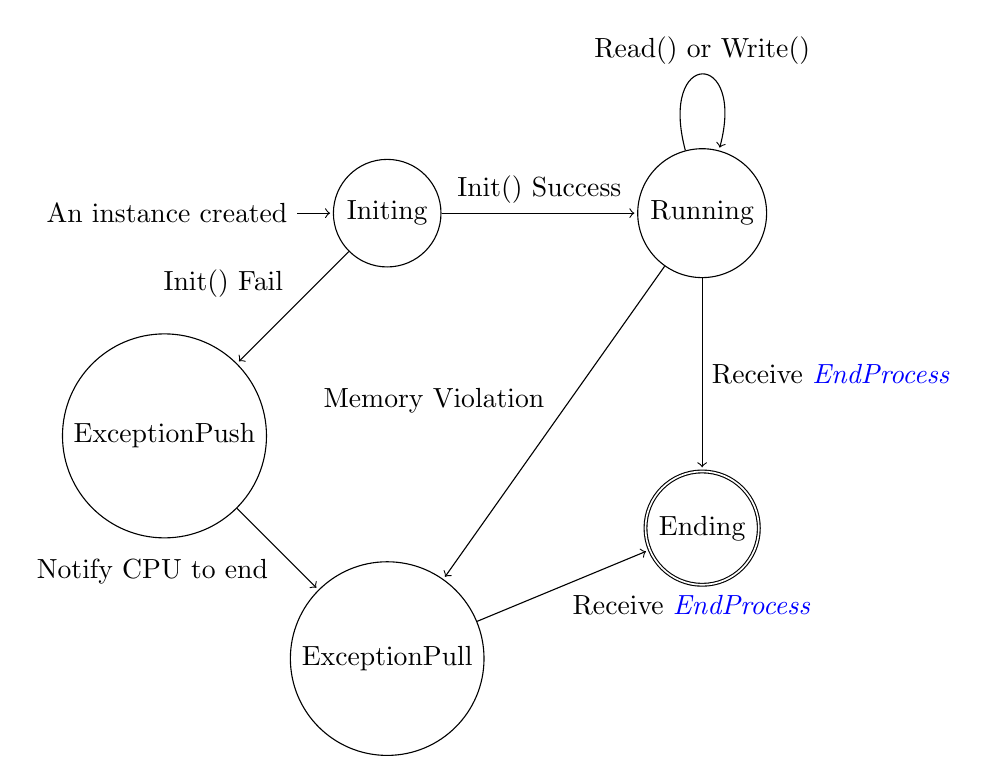
\begin{tikzpicture}[shorten >=1pt,node distance=4cm,on grid,auto,initial text=An instance created]
  \node[state,initial] (q_0) {Initing};
  \node[state] (q_1) [right=of q_0] {Running};
  \node[state] (q_2) [below left=of q_0] {ExceptionPush};
  \node[state] (q_4) [below right=of q_2] {ExceptionPull};
  \node[state,accepting](q_3) [below =of q_1] {Ending};

  \path[->] (q_0) edge node {Init() Success} (q_1)
                  edge node [swap] {Init() Fail} (q_2)
            (q_1) edge node {Receive \textit{\color{blue} EndProcess}} (q_3)
                  edge node [swap] {Memory Violation} (q_4)
                  edge [loop above] node {Read() or Write()} ()
            (q_2) edge node [swap] {Notify CPU to end} (q_4)
            (q_4) edge node [swap] {Receive \textit{\color{blue} EndProcess}} (q_3);
\end{tikzpicture}

Let me explain that: In the constructor of class \textit{\color{blue} Memory}, I initalize the state to \textit{\color{blue} MemoryIniting}. After calling the \textit{\color{blue} void Memory::Init(void)} function, if there is no error occurred, I change the state to \textit{\color{blue} MemoryRunning}. If there is an error occurred in the process of parsing a program file, I change the state to \textit{\color{blue} MemoryExceptionPush}, meaning that memory will not work and in the next time memory repares a respond for CPU request, it sends an error respond message which is indicated by \textit{\color{blue} MemoryError} and then changes state to \textit{\color{blue} MemoryExceptionPull} to wait the end message of CPU. I also handle memory violation by using this state. I just send a respond message which operation result is \textit{\color{blue} MemoryViolation} and then also changes state to \textit{\color{blue} MemoryExceptionPull}. So all errors will lead to this state. After pulling an \textit{\color{blue} EndProcess} message sent by CPU, memory just changes state to \textit{\color{blue} MemoryEnding} and terminates the child process.

\section*{Personal Experience}
In this well-designed project, I learn about important concepts of operating system. With this concepts, I could build a simple view of the internal work scheme of CPU and memory to build a solid foundation for understanding complicated concepts of operating system. In addition to that, I try to analyze and  split a project's requirements and implement each part progressively to finish a whole project. For example, I firstly build the memory part, parsing program files, and then test this part implementation by using all sample files. After finishing that, I make pipe communication works. After doing these, I have set a basic running environment for CPU. So I do the last missing part. I start to implement a small subset of instructions involved in the sample1.txt. After done the sample1.txt, I add some missing implemention of instructions in the sample2.txt. So for testing each sample file, I amend some missing implementation of instructions. After successfully testing all sample files, I noticed that there are still some instructions which are not covered in the sample files. So I add some test cases in the sample5.txt to cover all instructions. This progressively building process makes me focusing on implementing on each part and enhance the development efficiency because if I have done the previous part, I will test this part until it has no problem. In the implemtation of next part, I will not be affected by some bugs of previous part.
\end{document}
